\chapter[Scaling Laws and Efficiency]{Scaling Laws and Efficient Large Language Models}\label{chap:scaling}

\begin{learningbox}
In this chapter you will learn how  performance of language models scales with data and training effort.
Specifically, you will be able to:
\begin{itemize}[leftmargin=*, nosep]
    \item Explain how model performance relates to compute, data, and model size through {\em scaling laws}, and predict the effect of increasing one factor while holding the others fixed.
    \item Describe what techniques can be used to develop {\em smaller language models}, and analyze the tradeoff of using smaller models with respect to compute requirements and performance. 
    \item Recognize the difference between {\em inference-time compute} and training-time compute.
    \item Reflect on \emph{sustainable language models} and the environmental and privacy implications of large-scale deployment 
\end{itemize}
\end{learningbox}

\begin{comment}
Now that we have seen how to  design, train, and evaluate large language models, we will focus on performance: we will look beyond the models and observe general patterns related to the underlying resources required for creating them. We separate our discussion into four parts. First, we discuss how a model's performance can be predicted according to \emph{scaling laws} (Section~\ref{sec:scaling-laws}). Next, we turn to \emph{small language models} and the techniques that make them capable under resource budgets (Section~\ref{sec:small-models}). We then discuss \emph{inference-time compute}, where additional computation is spent at inference time rather than during training (Section~\ref{sec:inference-time}). Finally, we reflect on \emph{sustainable language models} and the environmental and privacy implications of large-scale deployment (Section~\ref{sec:sustainable}).
\end{comment}

\section{Scaling Laws: Compute, Data, Parameters}
\label{sec:scaling-laws}
There are three primary factors involved in the training of LLMs: \begin{enumerate*}[label=(\arabic*)]
    \item the amount of compute,
    \item the size of the dataset, and
    \item the size of the model.
\end{enumerate*}
Studies have shown that these three factors relate to the final performance of a model, measured as its loss on a held-out test set ($L$). This relation has been found to be  both smooth and predictable. The relationship takes the form of a \emph{power law}: as any of the three resources is increased, the loss decreases proportionally to a negative power of that resource. For instance, doubling the model size might reduce the loss by a factor of $2^{-\alpha}$ for some positive exponent $\alpha$. Because the behavior is predictable, we can estimate how much a model will improve (for instance, from doubling the training dataset size) \emph{before} committing to an expensive training run.

We define these three quantities ($C$, $D$, $N$)  as follows:
\begin{itemize}
    \item Compute ($C$): the total amount of arithmetic performed over the entire training run, measured in floating point operations (FLOPs). Note that this is a count of operations in total, not a rate per second. A widely used approximation relates it to the other two quantities as $C \approx 6ND$, since processing a single token touches each of the $N$ parameters roughly six times across the forward (twice) and backward pass (four times).
    \item Dataset size ($D$): the total number of tokens the model is trained on. Note that a token is a subword unit defined by the tokenizer, so the same corpus corresponds to different values of $D$ under different tokenizers. The count of $D$ is the number of tokens as they are used during the training run. When data is repeated over several epochs, the repeated tokens still add to $D$ but may yield diminishing returns compared to fresh data.
    \item Model size ($N$): the number of trainable parameters (weights) in the model architecture. This count usually refers only to the parameters that increase when scaling model depth, and therefore excludes the embedding matrix.
\end{itemize}
Training large models comes at considerable cost, usually in the realm of tens of millions of dollars, and up to months of compute time. Scaling laws allow us to predict whether a model will train well.

\begin{figure}[t]
    \centering
    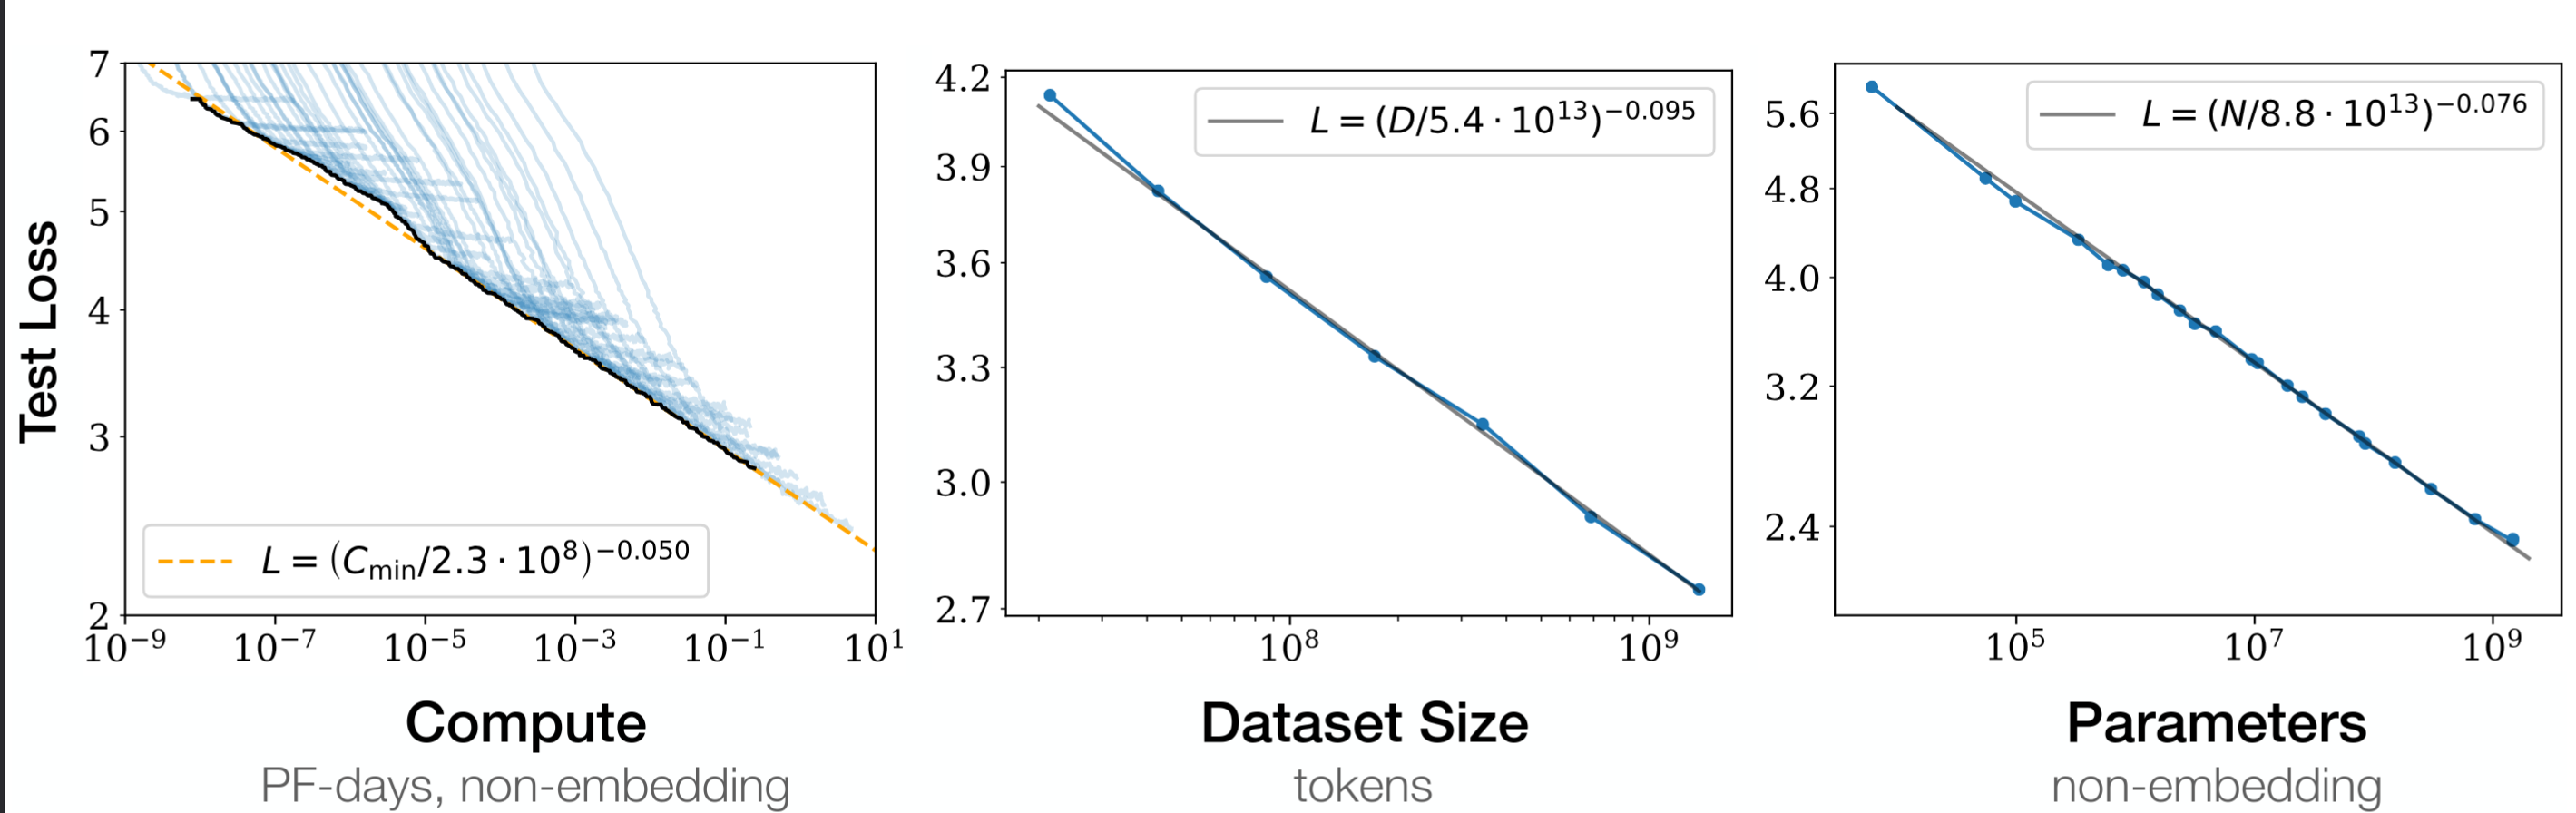
\includegraphics[width=0.9\linewidth]{part1/visuals/scaling.png}
    \caption{Loss on language modeling objective is a function of training compute, dataset size, and model size \citep{kaplan2020scalinglawsneurallanguage}.}
    \label{fig:scaling-law}
\end{figure}


\subsection{Kaplan Scaling Laws}
There are different empirical results for scaling laws that are found by fitting a function to empirical test data. For instance, in Figure~\ref{fig:scaling-law}, every point is a trained model on a fixed dataset with a similar experimental setup, while only changing the three primary variables $C,D,N$. In early 2020, \citet{kaplan2020scalinglawsneurallanguage} found how model performance is related to $C,D,N$. 
They estimated, following empirical observations, that the loss follows independent power laws rekated to the three main variables: $L(N) \propto N^{-\alpha_N}$ and $L(D) \propto D^{-\alpha_D}$, with $\alpha_N \approx 0.076$ and $\alpha_D \approx 0.095$. 

The individual power laws can be combined into a single optimizable equation, shown in Equation~\ref{eq:joint-power}. This relationship was assumed to be generic: it would apply well as models of loss behavior for ``other generative modeling tasks'' \citep[p. 5]{kaplan2020scalinglawsneurallanguage}. The authors further showed that, under no other constraints than compute budget, their derivations would point to optimal model size $N$, an ideal dataset size $D$, defined by optimal step size ($S$) and batch size ($B$).  

\begin{equation}
\label{eq:joint-power}
L(N, D) = \Big[ \Big(\frac{N_c}{N}\Big)^{\frac{\alpha_N}{\alpha_D}} + \frac{D_c}{D} \Big]^{\alpha_D}
\end{equation}

Specifically, they concluded that as the compute budget $C$ increases, model size $N$ should be increased  faster than data size $D$ ($N \propto C^{0.73}$ and $D \propto C^{0.27}$\footnote{$B\propto C^{0.24},\,S\propto C^{0.03},\, D=B\cdot S \propto C^{0.27}$}), leading to the development of large models such as GPT-3.  The negative exponents reflect diminishing returns: each doubling of model size or dataset size lowers the loss by only a few percent.  

At first glance, this recommendation seems to contradict the exponents themselves: since $\alpha_D > \alpha_N$, data scaling reduces the loss \emph{faster} than parameter scaling for the same relative increase in compute. The reason is that compute, not the resource itself, is the constraint: because $C \approx 6ND$, increasing $D$ consumes compute just as increasing $N$ does. This means that $N$ is with becoming a bottleneck with increasing likelihood. Hence, once the compute cost for $D$ is accounted for, allocating additional compute to $N$ yields a better return than allocating it to $D$. This means that the optimal allocation favors larger models.






\paragraph{Sample efficiency} 
A separate observation of \citet{kaplan2020scalinglawsneurallanguage} is that larger models are more \emph{sample-efficient}. For a fixed number of training tokens, a larger model reaches a lower loss, and to reach a given target loss it requires fewer tokens and fewer optimization steps than a smaller one. This effect is visualized in Figure~\ref{fig:sample-efficiency-tokens}.

\begin{figure}[t]
    \centering
    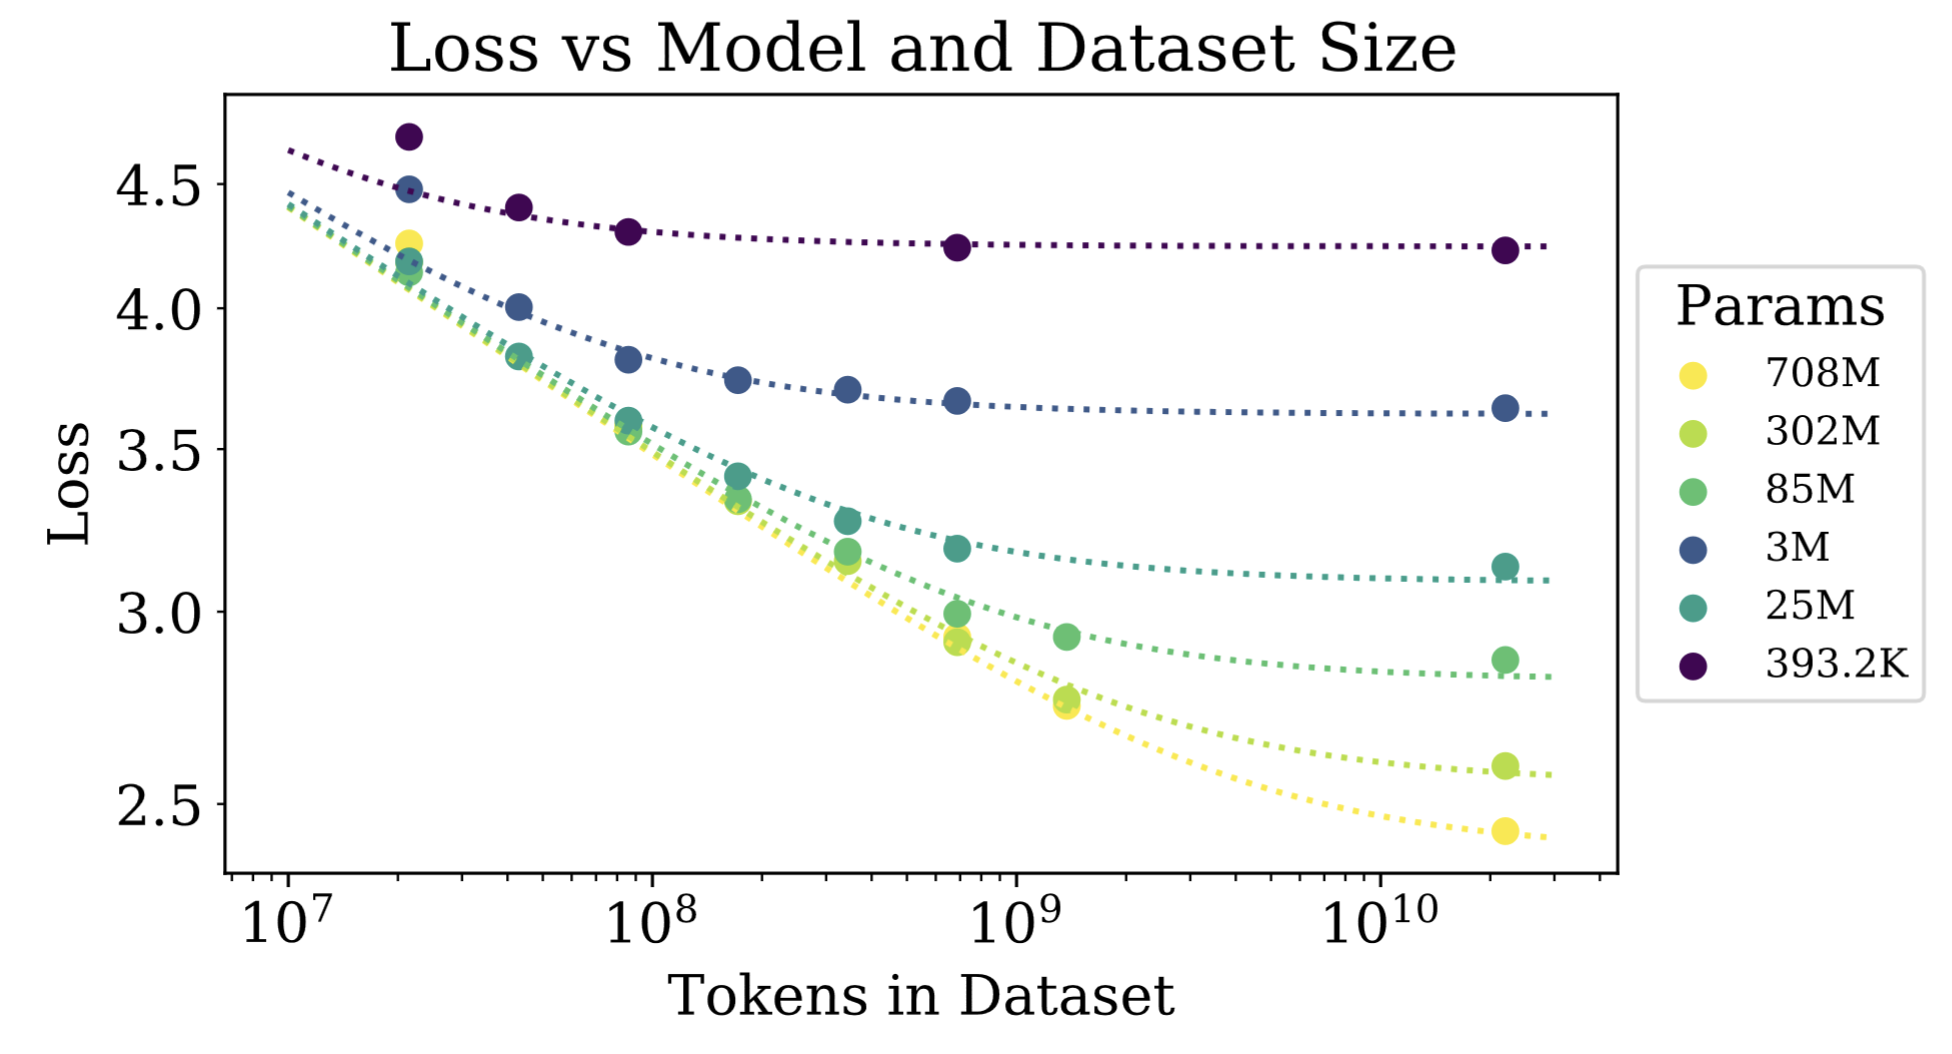
\includegraphics[width=0.7\linewidth]{part1/visuals/sample_efficiency_tokens.png}
    \caption{Larger models reach a given loss using fewer training tokens, illustrating greater sample efficiency \citep{kaplan2020scalinglawsneurallanguage}}
    \label{fig:sample-efficiency-tokens}
\end{figure}


\subsection{Chinchilla Scaling Laws}
In 2022, \citet{10.5555/3600270.3602446} reevaluated these findings with a model called Chinchilla, and found, surprisingly, that most large models at the time were severely undertrained. This discrepancy can be traced back to the methodology of \citet{kaplan2020scalinglawsneurallanguage}: their optimal allocation was extrapolated from the \emph{early}, non-converged training dynamics of many models rather than from runs trained to convergence, which systematically biased their conclusions toward larger models trained for fewer steps. 

The key insight from the Chinchilla study  was that for every doubling of the compute budget, both the model size $N$ and the number of training tokens $D$ should be increased in roughly equal proportions ($N \propto C^{0.5}$ and $D \propto C^{0.5}$). Their rule of thumb suggests training on approximately 20 tokens for every trainable parameter in the model to achieve compute optimality. This result has since been reproduced \citep{besiroglu2024chinchilla} and has been shown to be robust to sizable perturbations \citep{schaeffer2025evaluating}.

In their scaling laws, the loss is modeled as a function of the parameter count $N$ and the number of  tokens $D$ that have been trained on, as follows:
\begin{equation}
    L(N,D) = E + \frac{A}{N^{\alpha}} + \frac{B}{D^{\beta}}
\end{equation}

The first term $E$ captures the irreducible loss, corresponding to the entropy of natural text. The second term $\frac{A}{N^{\alpha}}$ captures the sub-optimality of a model with finite parameters $N$, and the final term $\frac{B}{D^{\beta}}$ captures the sub-optimality due to training on a finite number of tokens $D$. Although $\alpha$ and $\beta$ here play the same role as Kaplan's $\alpha_N$ and $\alpha_D$ (the exponents governing how the loss falls off with model size and data) they are a different parameterization: they are fit jointly within this two-term form and therefore take different values. Fitting the Chinchilla scaling function on more than 400 models found the following parameter estimates:
\begin{equation}
    E \approx 1.69, \quad A \approx 406.4, \quad B \approx 410.7, \quad \alpha \approx 0.34, \quad \beta \approx 0.28
\end{equation}

By optimizing this loss function under the constraint of a fixed compute budget $C$ (recall $C \approx 6ND$), we can derive the compute-optimal model size $N_{opt}$ and data size $D_{opt}$ for any budget $C$:
\begin{equation}
    N_{opt}(C) = G \left( \frac{C}{6} \right)^a, \quad D_{opt}(C) = \frac{1}{G} \left( \frac{C}{6} \right)^b
\end{equation}
where $G=\big(\frac{\alpha A}{\beta B}\big)^{\frac{1}{\alpha + \beta}}$ is a constant, $a = \frac{\beta}{\alpha + \beta} \approx 0.45$ and $b = \frac{\alpha}{\alpha + \beta} \approx 0.55$. 

Note that $a$ and $b$ are not independent: by construction $a+b=1$. This follows directly from $C \approx 6ND$, since taking logarithms gives $\log C = \log 6 + \log N + \log D$. Writing $N_{opt} \propto C^a$ and $D_{opt} \propto C^b$, this becomes $\log C = \text{const} + a \log C + b \log C$, which can only hold for all $C$ if $a+b=1$. The same constraint applies to Kaplan's exponents ($0.73 + 0.27 = 1$). The difference for Chinchilla was \emph{how} the budget is split between $N$ and $D$.

% \paragraph{How constant is the ``20''?} The ratio is only \emph{approximately} fixed: since $D_{opt}/N_{opt} \propto C^{\,b-a}$ with $b-a \approx 0.1$, each tenfold increase in the compute budget multiplies the optimal token-to-parameter ratio by only $10^{0.1} \approx 1.26$, a change of about $26\%$ per order of magnitude. Over the practically relevant range this leaves the ratio in the ``tens of tokens per parameter'' band, which \citet{10.5555/3600270.3602446} rounded to the memorable constant $20$. 

This rule is approximately \emph{linear} because $N_{opt}$ and $D_{opt}$ grow with the compute budget $C$ at almost the same rate: their exponents $a \approx 0.45$ and $b \approx 0.55$ are close, so the ratio $D_{opt}/N_{opt}$ stays near a constant value of roughly $20$ across many orders of magnitude of compute. 
The value is best understood as an empirical calibration anchored on real compute-optimal runs rather than a number that results cleanly from the fitted coefficients. The Chinchilla model itself (70B parameters trained on 1.4T tokens) sits exactly at $D/N = 20$. Table~\ref{tab:token-param} shows several well-known models relative to this rule. Models below the ratio are \emph{undertrained} (too large for their token budget), while models far above it are deliberately \emph{overtrained} to obtain a small model that is cheap to run at inference time. Earlier flagship models such as GPT-3 and Gopher fall well below the line ($D/N \approx 1$--$2$): they were made very large but trained on comparatively too few tokens.
% In the models Chinchilla used, to spend a compute budget optimally one should train on about $20$ tokens for every parameter; a compute-optimal $10$B-parameter model, for example, calls for on the order of $200$B training tokens.
% This was the central correction over the earlier recommendation of \citet{kaplan2020scalinglawsneurallanguage}, under which models were made very large but trained on comparatively too few tokens. 
It is worth stressing that $D \approx 20N$ is optimal only for minimizing the \emph{training} loss at a fixed training budget. When a model will later serve many inference requests, it is often deliberately \emph{over-trained} on far more than $20$ tokens per parameter, trading additional training cost for a smaller model that is cheaper to run at inference time. LLaMA-3 8B, for instance, is trained on roughly $1900$ tokens per parameter. This deliberate extreme over-training is chosen so that a small model still reaches a low loss, and is cheap to run during inference. 

\begin{table}
    \centering
    \begin{tabular}{lrrrl}
        \toprule
        Model & $N$ & $D$ & $D/N$ & Regime \\
        \midrule
        Gopher \citep{rae2021scaling}            & 280B & 300B & $\approx 1$    & undertrained \\
        GPT-3 \citep{brown2020language}          & 175B & 300B & $\approx 1.7$  & undertrained \\
        Chinchilla \citep{10.5555/3600270.3602446} & 70B  & 1.4T & $20$           & compute-optimal \\
        LLaMA-1 7B \citep{touvron2023llama1}     & 7B   & 1.0T & $\approx 143$  & overtrained \\
        LLaMA-2 7B \citep{touvron2023llama}      & 7B   & 2.0T & $\approx 286$  & overtrained \\
        LLaMA-3 8B \citep{grattafiori2024llama3herdmodels} & 8B   & 15T  & $\approx 1875$ & overtrained \\
        \bottomrule
    \end{tabular}
    \caption{Token-to-parameter ratios of several well-known models relative to the Chinchilla rule of thumb $D \approx 20N$.}
    \label{tab:token-param}
\end{table}


% Proceed with rest of section by introducing the four phenomena related to model scaling.
The picture so far is fairly clean: test loss falls smoothly, monotonically, and predictably with compute, data, and parameters. However, in practice, various factors influence our results. We discuss four phenomena that each probe a different edge of that picture:
\begin{enumerate*}[label=(\arabic*)]
    \item compute-optimal curves,
    \item emergent abilities,
    \item inverse scaling, and
    \item grokking.
\end{enumerate*}
    

\subsection{Compute-Optimal Curve}
Computer hardware and energy are finite resources. A practical question is how to split a fixed compute budget $C$ between model size $N$ and dataset size $D$ to obtain the best possible model. Scaling laws answer this through the \emph{compute-optimal frontier}: the allocation of $C$ that minimizes the loss.

This frontier is located empirically with the \emph{IsoFLOP} method \citep{10.5555/3600270.3602446}, shown in Figure~\ref{fig:isoflop}. For various model sizes, we choose the number of training tokens such that the final FLOPs is a constant. The learning rate is adjusted using a cosine annealing schedule, with the cosine cycle length is set to match the target FLOP count. We find a clear valley in loss, meaning that for a given FLOP budget there is an optimal model size to train (left). Using the location of these valleys, we project optimal model size and number of tokens for larger models (center and right). In green, we show the estimated number of parameters and tokens for an optimal model trained with the compute budget of Gopher. For a fixed FLOP budget we train several models of different sizes: a model that is too small underfits, while a model that is too large is forced to train on too few tokens, so the resulting curve of loss against model size is U-shaped. Its minimum identifies the compute-optimal model size $N_{opt}$, from which the matching token count $D_{opt} = C / 6N_{opt}$ follows via $C \approx 6ND$. Fitting a parabola to each such curve locates this minimum, and repeating the procedure across budgets finds how $N_{opt}$ and $D_{opt}$ grow with compute. 

This parabola fitting must be done with care, and the simplification introduces systematic biases in the estimated optimum \citep{czech2026problemschinchillaapproach2}. These biases persist even on noise-free synthetic data and stem from three sources: (1) spacing the sampled model sizes too coarsely, (2) sampling that fails to locate the true minimum symmetrically, and (3) the genuine asymmetry of the loss surface, which a symmetric parabola cannot represent. At the scale of Llama-3, they estimate that such biases waste on the order of \$1.4M of compute. As a remedy, they recommend fitting the parametric loss model $L(N,D) = E + A/N^{\alpha} + B/D^{\beta}$ directly---Chinchilla Approach 3, the same form we used above to derive the $D \approx 20N$ rule---with a numerically robust optimizer, rather than reading the optimum off fitted parabolas.

Complementary views on scaling \citep{paquette2024}  study analytically solvable models (power-law random features trained with one-pass stochastic gradient descent) instead of fitting curves to trained models. They find that the compute-optimal exponent is not a single universal constant, but that  the data-complexity/target-complexity plane instead splits into four primary phases (plus three sub-phases), each with its own exponent governing how $N_{\mbox{opt}}$ grows with compute.  The answer to the question which allocation rule to apply, and whether a fixed {\em 20 tokens per parameter} is even the right shape, depends on the  regime of the  problem.


\begin{figure}
    \centering
    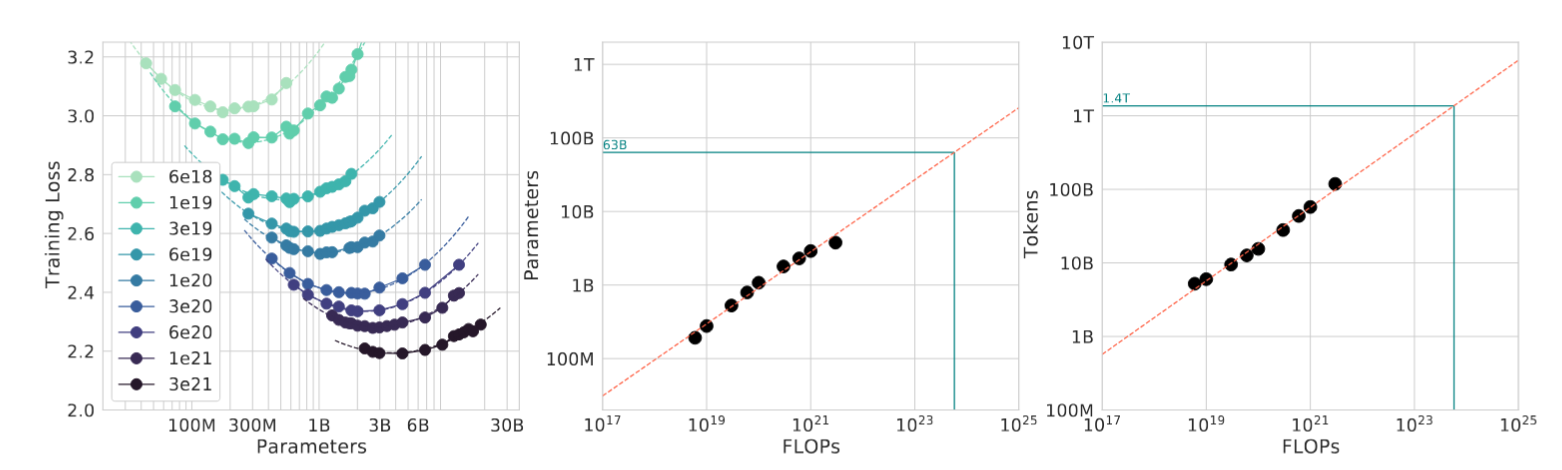
\includegraphics[width=\linewidth]{part1/visuals/isoflop.png}
    \caption{IsoFLOP curves  \citep{10.5555/3600270.3602446}}
    \label{fig:isoflop}
\end{figure}


\paragraph{Scaling for finetuning}
The preceding works studied how pretraining scales. Do these scaling laws also govern finetuning? \citet{zhang2024when} study this question for both full-model finetuning, which updates all of the model's weights, and parameter-efficient finetuning (PEFT), which freezes the pretrained weights and trains only a small set of added parameters (as in LoRA) \citep{hu2021lora}. The lesson most relevant to compute budgeting is that finetuning performance improves  more from scaling the size of the \emph{base model} than from collecting additional finetuning data, while adding more trainable PEFT parameters helps little. In practice, a task that underperforms is usually better served by starting from a larger pretrained model than by enlarging the adapter or gathering more finetuning examples.


\subsection{Emergent Abilities}
Some of the most interesting phenomena in LLM scaling are \emph{emergent abilities}: capabilities that are not present in smaller models but that appear suddenly as model size or compute cross a certain threshold \citep{wei2022emergent}. Examples include multi-step reasoning, few-shot translation, and specialized coding tasks, as shown in Figure~\ref{fig:emergent-abilities}. The ability to perform a task via few-shot prompting is emergent when a language model achieves random performance until a certain scale, after which performance significantly increases to well-above random.

\begin{figure}
    \centering
    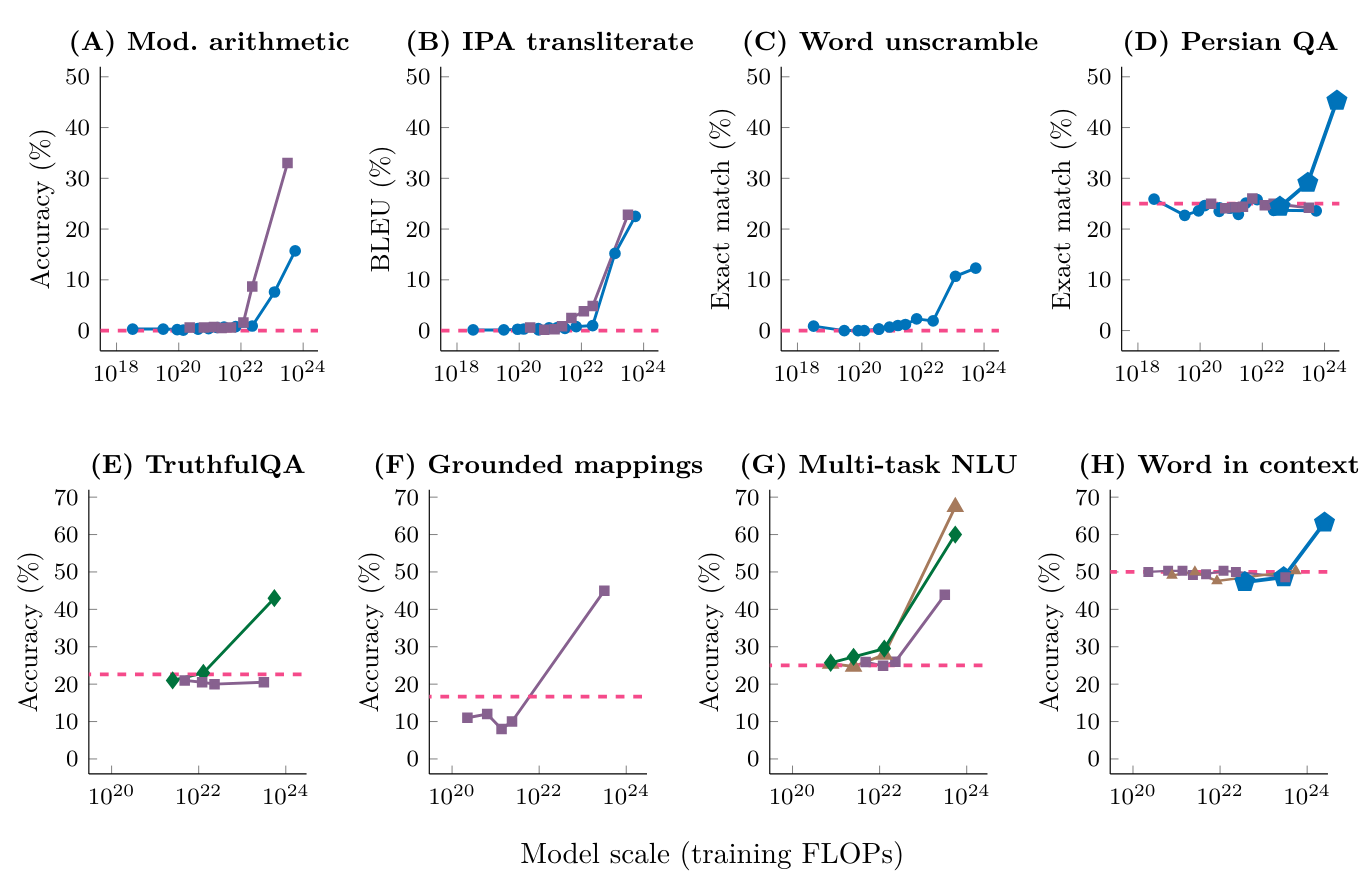
\includegraphics[width=0.9\linewidth]{part1/visuals/emergent.png}
    \caption{Eight examples of emergence in the few-shot prompting setting, each point is a separate model \citep{wei2022emergent}.}
    \label{fig:emergent-abilities}
\end{figure}


However, the  suddenness of the appearance has been contested. \citet{schaeffer2023emergent} argue that emergent abilities might be a mirage caused by the choice of evaluation metrics. For instance, in Figure~\ref{fig:emergent}, we see that while non-smooth discrete metrics (such as accuracy or exact match) show sharp jumps---they are non-smooth, after all---underlying metrics (such as the cross-entropy loss or token-level probability) follow a smooth, predictable power law across scales. 
% Top: When performance is measured by a nonlinear metric (e.g., Accuracy), performance appears sharp and unpredictable on longer target lengths. Bottom: When performance is instead measured by a linear metric (e.g., Token Edit Distance), the family exhibits smooth, predictable performance improvements 




\begin{figure}
    \centering
    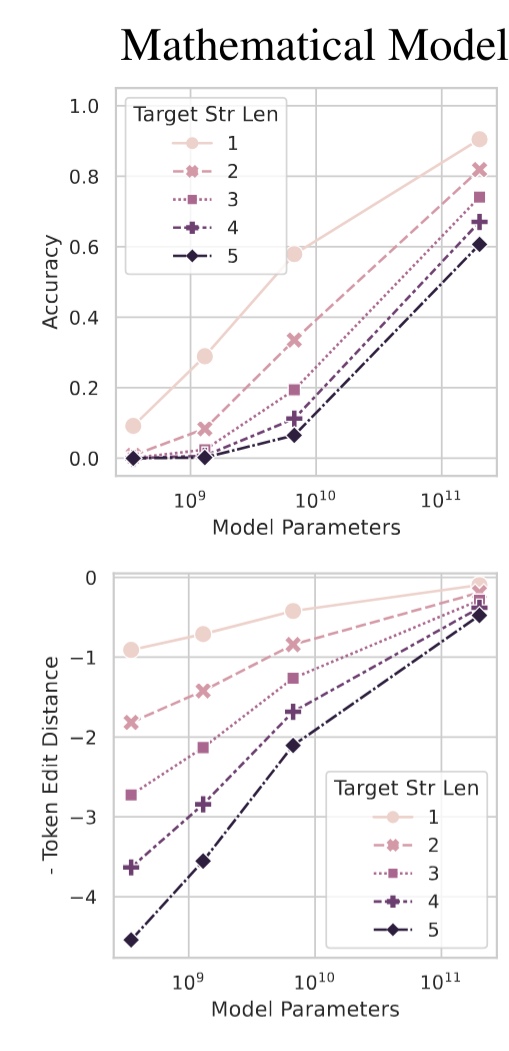
\includegraphics[width=0.3\linewidth]{part1/visuals/token_edit.png}
    \caption{Claimed emergent abilities evaporate upon changing the metric from a nonlinear (top) to a smooth (bottom) metric \citep{schaeffer2023emergent} }
    \label{fig:emergent}
\end{figure}







\subsection{Inverse Scaling}
While most tasks improve with scale, some exhibit \emph{inverse scaling}, where larger models perform worse or develop stronger biases. This may happen in tasks where a distractor answer is more probable according to the language modeling objective than the correct answer, leading larger (and more confident) models to consistently choose the wrong option \citep{mckenzie2023inverse, michaelov-bergen-2023-emergent}. 

An example of inverse scaling is \emph{hindsight neglect}, a task that tests whether a bet was worth taking based on its expected value. In case the expected value is positive, the model should respond with {\em yes}, and in case of a negative expected value it should respond with {\em no}. The situation is as follows. The model is only shown few-shot examples where the actual outcome always matches the expected value (that is, the bettor won money when the expected value was positive and lost money when the expected value was negative). The model is then asked a question about whether it was correct to take a bet where the expected value and the actual outcome do not match. Hindsight neglect tests whether models can correctly generalize from instructions when the few-shot examples are correctly-labeled but misleading. Repetitive algebra tests how models respond to simple algebra questions when given a specific pattern of correctly-labeled few-shot examples. Figure~\ref{fig:negative-scaling} shows that models generally start around random performance, but fall below random performance at around $10^{22}$ training FLOPs. 

\begin{figure}
    \centering
    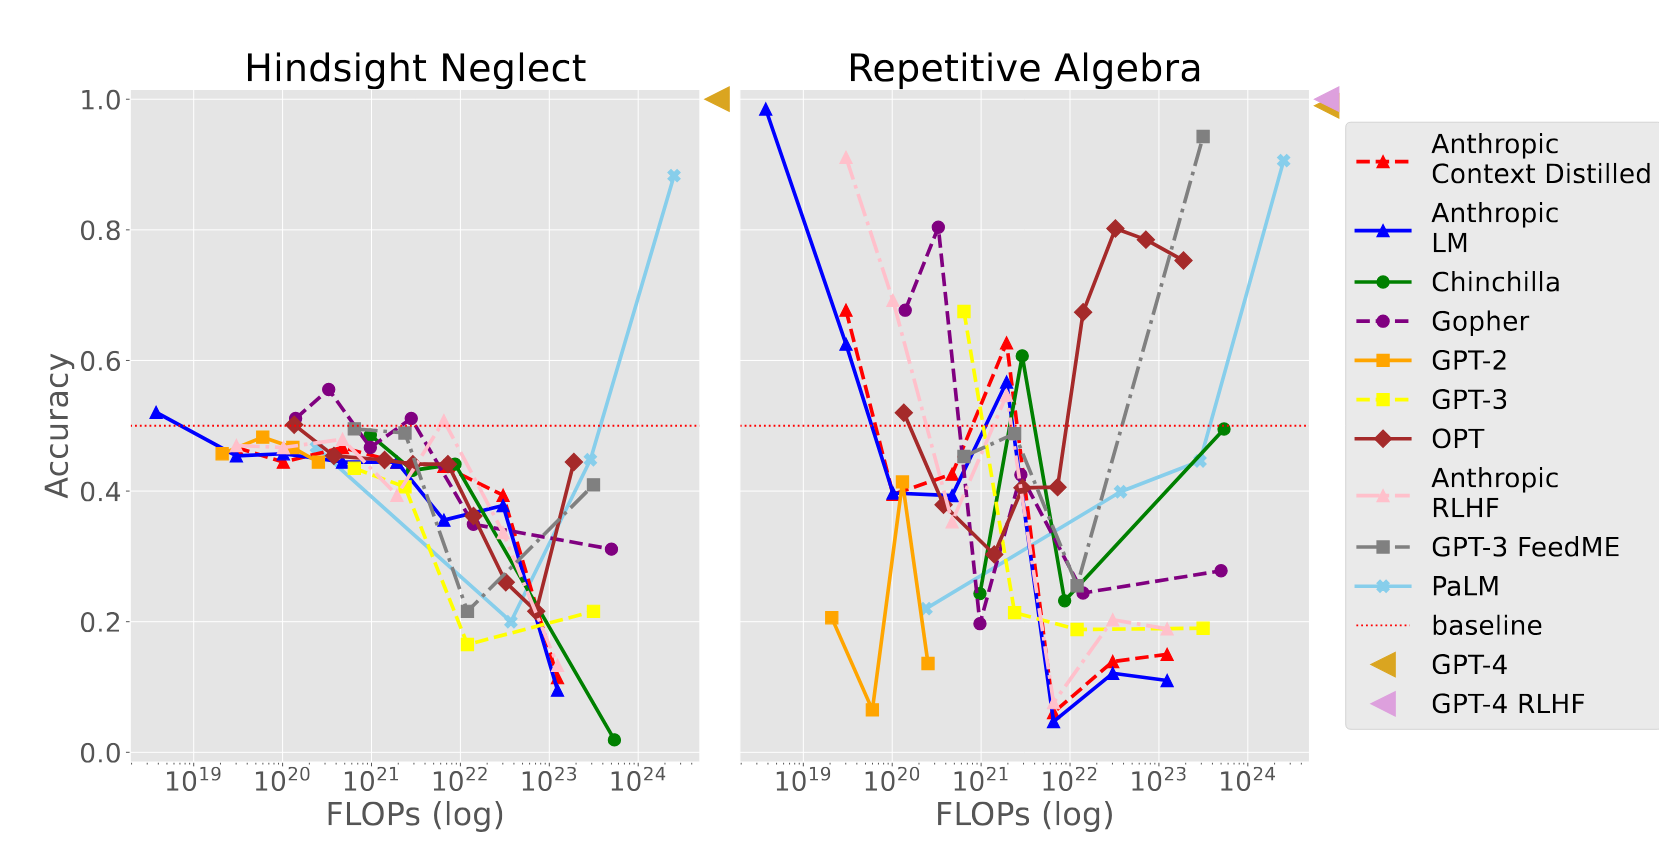
\includegraphics[width=0.8\linewidth]{part1/visuals/negative_scaling.png}
    \caption{Scaling behavior for the Hindsight Neglect (left) and Repetitive Algebra (right) tasks \citep{mckenzie2023inverse}}
    \label{fig:negative-scaling}
\end{figure}


\subsection{Grokking}
Grokking is a relatively recent paradox in statistical learning theory. This theory holds that, conventionally,  when a large model is presented with a small dataset, it will overfit, due to memorization of the examples. Grokking, then, occurs when we continue to train this too-large model, and, after much more training, the model suddenly finds a generalizing solution \citep{power2022grokkinggeneralizationoverfittingsmall}. 

While originally observed on small algorithmic tasks, such as modular addition, the grokking phenomenon suggests that scaling the number of training steps (over-training) can lead to qualitative shifts from memorization to understanding, even without increasing the dataset size $D$, see Figure~\ref{fig:grokking}.

\begin{figure}
    \centering
    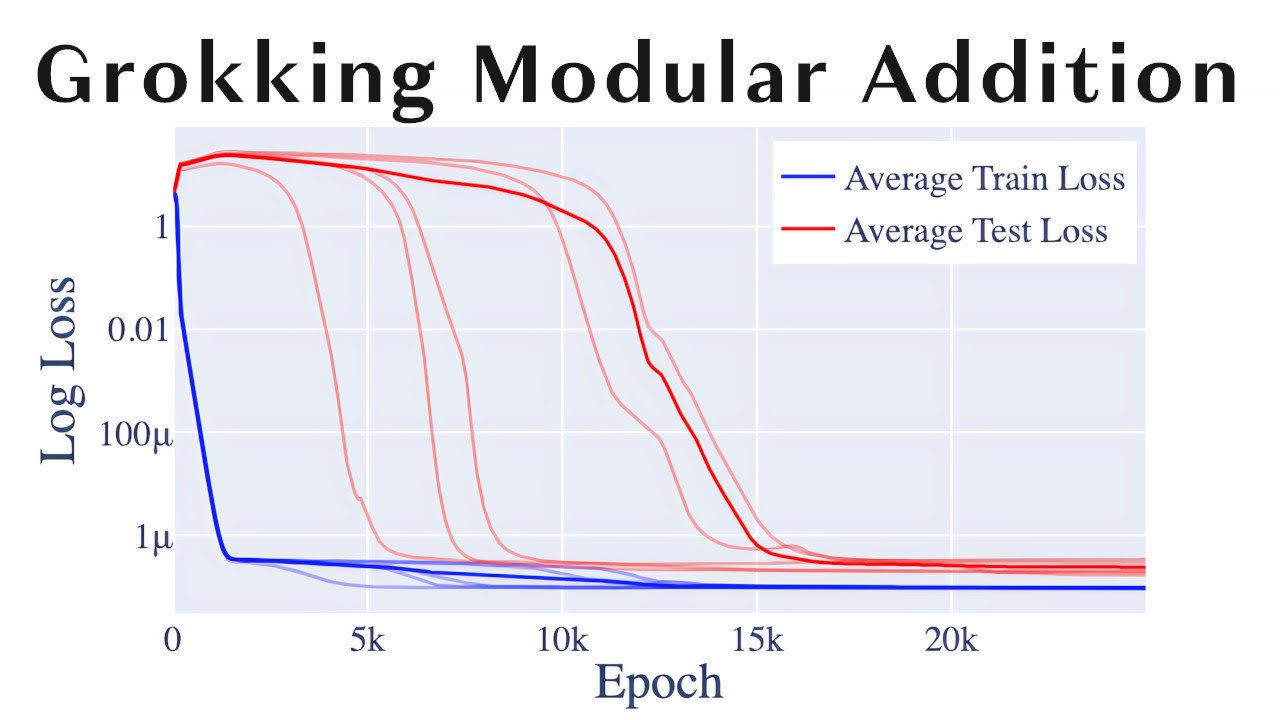
\includegraphics[width=.6\linewidth]{part1/visuals/Grokking_modular_addition.jpg}
    \caption{Early memorization of the training set (blue) versus late generalization (red: grokking) on a modular addition task \citep{nanda2023progress}}
    \label{fig:grokking}
\end{figure}


The figure shows a data wall that initially limits  scaling as the data is running out \citep{villalobos2024position}, but later, after much more training, the model groks a generalizing solution.  

Grokking is relevant to language modeling since we are rapidly running out of high-quality human text on the internet to satisfy the requirements on data $D$ of Chinchilla scaling for next-generation models. Because of these inherent limits, researchers are looking beyond simple scaling of $D$. As an alternative, we can look at a variety of these new frontiers:
%\begin{enumerate*}[label=(\arabic*)]
%    \item 
(1) better architectural efficiency (such as Mixture of Experts),
%    \item 
(2) inference-time scaling (such as  giving models more compute during inference to {\em think}, as seen in OpenAI's o-series), or
%    \item 
  (3)  synthetic data generation (Chapter~\ref{chap:synthetic-data}).
%\end{enumerate*}


\section{Small Language Models}
\label{sec:small-models}
As the requirements for compute and data continue to grow, there is an increasing interest in \emph{small language models} (SLMs): models that are small enough to run on consumer hardware or even mobile or edge devices while maintaining high performance. These models are often developed using techniques that optimize for efficiency without sacrificing too much performance.

To understand the deployment landscape for these models, it is helpful to categorize common types of compute infrastructure:
\begin{itemize}
    \item Datacenters: High-performance GPUs (such as NVIDIA H100s) and TPUs, primarily used for {\em pretraining} large models and hosting high-throughput inference APIs.
    
    \item Consumer Hardware: Standard desktop GPUs and high-end CPUs, where SLMs can be affordably {\em finetuned} or run locally by individual users.
    
    \item Edge Devices: Mobile phones, Internet-of-Things devices, and laptops, which are increasingly equipped with Neural Processing Units (NPUs) specifically designed for low-power, efficient on-device {\em inference}.
\end{itemize}

To fit models into the latter constrained environments, optimization techniques  focus on speeding up throughput, reducing latency, reducing memory usage, and increasing sample efficiency. The techniques for achieving these goals can be grouped into two categories: (1) model-centric optimization, which targets the architecture of the models and their optimization approaches, and (2) data-centric optimization, which targets the data used to train the models. We will discuss both categories.

\subsection{Model-centric Optimization}
First we discuss the model-centric optimization techniques. 
We introduce the following techniques that allow for efficient training of smaller models, while still maintaining high task performance.
Model-centric techniques can focus on pretraining/finetuning or inference.

\subsubsection{Reducing Pretraining Cost}

\paragraph{Parameter-Efficient Fine-Tuning (PEFT)}

Methods such as {\em Low-Rank 
Adaptation} 
(LoRA) \citep{hu2021lora} allow for adapting a large model to a new task by  training only a tiny fraction (often $<1$\%) of its parameters \citep{lialin2023scaling}. The key observation is that the weight update learned during finetuning has a low {\em intrinsic rank}: although a pretrained weight matrix 
$W_0 \in \mathbb{R}^{d \times k}$
is full-rank, the change $\Delta W$ needed to adapt it to a new task can be approximated well by a low-rank matrix. Instead of updating $W_0$ directly, LoRA freezes it and represents the update as a product of two small matrices,
\begin{equation}
    W = W_0 + \Delta W = W_0 + B A, \qquad B \in \mathbb{R}^{d \times r}, \;\; A \in \mathbb{R}^{r \times k}
\end{equation}
where the rank $r \ll \min(d, k)$. For an input $x$, the modified forward pass becomes
\begin{equation}
    h = W_0 x + \frac{\alpha}{r}\, B A x,
\end{equation}
where $\alpha$ is a constant scaling factor that controls the magnitude of the update, roughly similar to a learning rate in standard training. This is visualized in Figure~\ref{fig:lora}. We compute weight updates only for $A$ and $B$, reducing the number of trainable parameters from $d \times k$ to $r(d + k)$. At initialization $A$ is drawn from a random Gaussian and $B$ is set to zero, so $\Delta W = 0$ and training starts from the pretrained model. Because $\Delta W$ can directly be merged back into $W_0$ after training, LoRA adds no inference latency, and a single base model can be served with many small, swappable task-specific adapters. 

\begin{figure}[t]
    \centering
    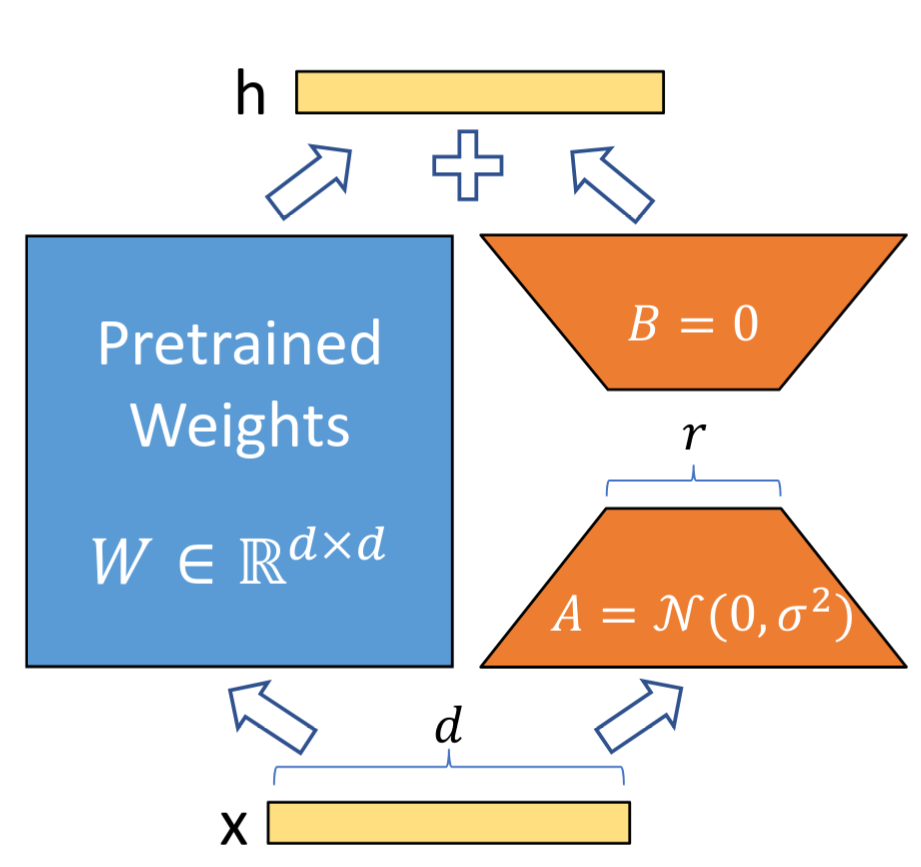
\includegraphics[width=.45\linewidth]{part1/visuals/lora.png}
    \caption{Low-Rank Adaptation reparametrization \citep{hu2021lora}. During finetuning, only $A$ and $B$ are trained}
    \label{fig:lora}
\end{figure}    

\paragraph{Architectural Innovations}
A second family of techniques changes the model architecture itself so that it is cheaper to run, rather than compressing a fixed architecture after the fact. Two influential examples are Grouped-Query Attention and Mixture of Experts.

\textit{Grouped-Query Attention} (GQA) \citep{ainslie-etal-2023-gqa} targets the memory bandwidth bottleneck of autoregressive decoding. In standard \emph{multi-head attention} (MHA), every query head has its own key and value matrix, which we all need to use for computing attention scores. At the other extreme, \emph{multi-query attention} (MQA) lets all query heads share a single key/value head, which shrinks the computation  but can hurt expressive quality and training stability. GQA interpolates between these two: the query heads are divided into $g$ groups, and all heads within a group share one key/value head. With $g = 1$ it is equivalent to MQA, and with $g$ equal to the number of heads it is equivalent to MHA, so $g$ trades quality against memory usage. Often, GQA is combined with the KV-caching optimizations discussed next in Section~\ref{sec:small-models}, and it is now the default attention variant in many open-weight models.

\textit{Mixture of Experts} (MoE) \citep{shazeer2017outrageouslylargeneuralnetworks} decouples the total number of parameters from the compute spent per token. Instead of a single dense feed-forward block in each layer, a MoE layer contains many parallel ``expert'' sub-networks together with a lightweight \emph{gating network} (router) that activates only a small number of experts (typically the top-$1$ or $2$) for each token. Because only the chosen experts perform computation, the per-token cost stays close to that of a single dense block even as the total parameter count (and hence the model's overall capacity) grows by an order of magnitude or more \citep{JMLR:v23:21-0998}. 

This \emph{sparse activation} is why models such as Mixtral and many recent frontier systems can have hundreds of billions of total parameters while activating only a fraction of them per token. The trade-offs are (1) that all experts must still be held in memory, (2) that the load must be balanced across experts (often via an auxiliary loss) so that no expert is over- or under-used, and (3) that routing introduces additional engineering complexity. The MoE architecture is visualized in Figure~\ref{fig:moe}, which shows a top-$k$ routing mechanism, configured with $k=2$, where the gating function selects the two highest-scoring FFN experts for each token based on the router. The selected experts are evaluated in parallel, with their outputs aggregated using weighted summation \citep{zhang2025mixtureexpertslargelanguage}. 

\begin{figure}[t]
    \centering
    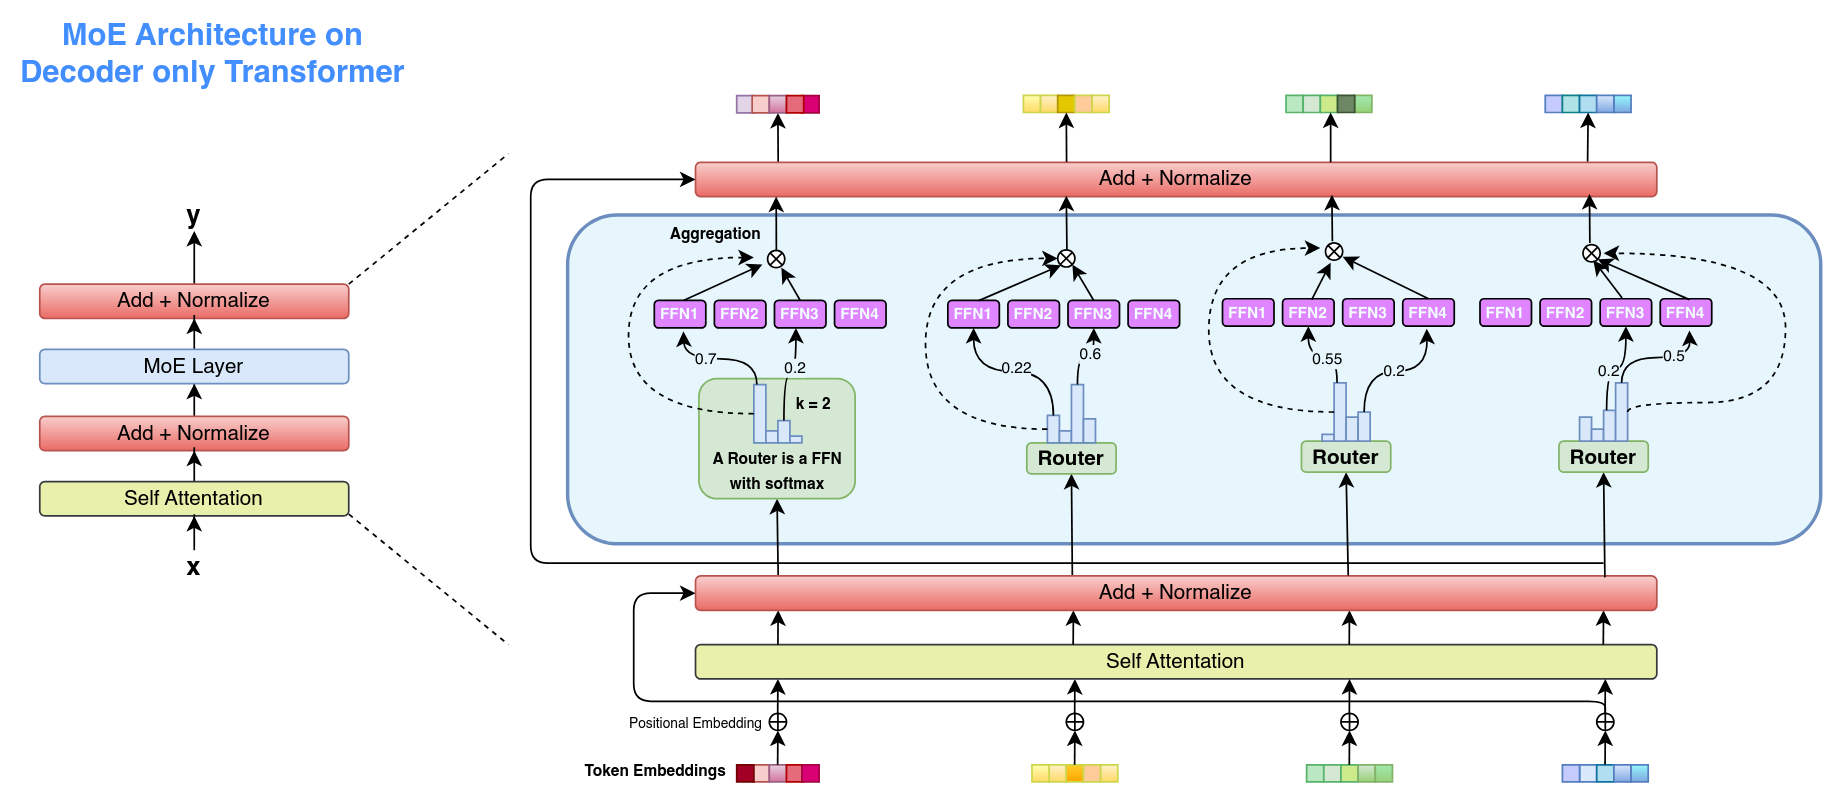
\includegraphics[width=.95\linewidth]{part1/visuals/moe.png}
    \caption{Illustration of the sparsely gated Mixture of Experts (MoE) architecture on top of a decoder-only transformer \citep{zhang2025mixtureexpertslargelanguage}}
    \label{fig:moe}
\end{figure} 

\paragraph{Knowledge Distillation}
A large teacher model is used to train a smaller student model by encouraging the student to match the teacher's output distribution \citep{gu2023minillm, xu2024survey}. Crucially, the student learns from the teacher's full \emph{soft} probabilities (typically softened with a temperature) rather than only the single correct answer. These soft targets carry richer information: for instance, which wrong answers the teacher considers plausible. This lets the student approach the teacher's quality at a fraction of its size. The same idea underpins  the synthetic-data generation discussed below, where a frontier model effectively acts as the teacher, generating high-quality training data for a smaller student model.


\subsubsection{Reducing Inference Cost}
Once a model is trained, it can be further optimized for deployment at inference time. Whereas training-time techniques focus on reducing the cost of producing the model, inference-time techniques target the cost of \emph{using} it: the throughput (tokens generated per second), the latency (time to the first and each subsequent token), and the memory footprint required to serve a request. We discuss several techniques that are commonly used to reduce inference cost, which can be applied to both large and small models.

\paragraph{Key--Value (KV) Caching} During autoregressive generation, the model produces one token at a time, and each new token attends to all previous tokens. Recomputing the attention keys and values for the entire context at every step is quadratically expensive. However, when we predict a new token, the context remains the same. Instead of recomputing the attention values, we can store the key and value vectors of past tokens in a \emph{KV cache} and reuse them. This turns per-step attention into a linear-cost lookup. This is the basic optimization that makes decoding practical, but it comes at a cost: the cache grows linearly with both sequence length and batch size and quickly dominates memory usage for long contexts. This problem has motivated both the architectural choices above (GQA and MQA shrink the cache by sharing key/value heads across query heads) and dedicated memory-management schemes such as \emph{PagedAttention}, which stores the cache in non-contiguous blocks to reduce fragmentation and enable higher serving throughput \citep{kwon2023efficient}.

\paragraph{Pruning} A more extreme method for reducing model size is to consider removing redundant or less important connections in the neural network  \citep{ma2023llm}. Pruning can be \emph{unstructured} (zeroing out individual weights) or \emph{structured} (removing entire neurons, attention heads, or layers); the latter yields concrete speedups on standard hardware, whereas the former requires sparsity-aware kernels to realize its benefits.

\paragraph{Quantization} Another method of saving memory during inference is to reduce the size of the matrix that needs to be loaded into memory. Rather than making the matrix dimensions smaller, we can also lower the precision of weights entries (e.g., from 16-bit to 8-bit or 4-bit numbers). This significantly reduces memory usage and speeds up inference. However,  in principle, lower precision means lower performance. The same idea can also be applied to the KV cache itself to keep long contexts in memory. Quantization is a frequently used approach \citep{dettmers2022gpt3, dettmers2023case, xiao2023smoothquant}. 

Alternatively, rather than casting all weights to the same precision, \emph{mixed precision} modes have been proposed, with different levels of numerical precision for different parts of the computation, to balance speed and stability \citep{micikevicius2017mixed}. This approach may suffer from non-deterministic results due to numerical instabilities \citep{yuan2025understanding}.

\paragraph{Speculative Decoding} A key technique for optimizing inference efficiency is \emph{speculative decoding} \citep{leviathan2023fast}. This approach uses a small draft model to generate multiple tokens quickly, which are then verified in parallel by a larger target model. This allows for faster inference (up to 2-3 fold speedup) without sacrificing the quality of the larger model, effectively leveraging the different points on the scaling curve.



\subsection{Data-centric Optimization}
In addition to model-centric approaches, the  literature emphasizes that data quality and curation are often more important than the size of the dataset when training efficient models \citep{luo-etal-2025-survey}. Small models can  perform  well if they are trained on highly curated, high-quality data. Hence, it is important to create a good data recipe, in addition to an efficient model architecture. Data-centric techniques broadly fall into two camps: \emph{selecting} the most useful parts from a broader pool of data, and \emph{generating} new synthetic data where good data is scarce.

\subsubsection{Data Selection and Curation}
Rather than training on all available text, a growing body of work shows that carefully choosing \emph{which} data to train on, and in what proportions, yields better models for the same compute budget. For pretraining, NVIDIA's \emph{CLIMB} framework \citep{diao2026nemotron} embeds a large corpus into a semantic space, clusters it, and then iteratively searches for the data mixture that minimises proxy-model loss. The resulting \emph{ClimbMix} dataset (400B tokens) lets a sub-billion-parameter model outperform comparable models trained on far larger but unfiltered corpora. The same principle applies at the finetuning stage: \emph{LIMA} \citep{zhou2023lima} shows that supervised finetuning on only $1{,}000$ carefully curated prompt--response pairs is enough to produce a strong instruction-following model, supporting the view that most knowledge is acquired during pretraining and that alignment mainly teaches the model a desired response \emph{style}.

\subsubsection{Synthetic Data Gathering}
When suitable data does not exist, it can be generated. The {\em Textbooks Are All You Need} approach, used for models such as Microsoft's Phi series \citep{gunasekar2024textbooks}, demonstrates that training on clean, synthetic textbook-quality data can allow a relatively small model of 1.3B parameters to outperform models ten times its size. 

Such pipelines typically rely on frontier models to generate the data, combined with {\em LLM-as-a-judge} scoring to filter for the most accurate and educational examples, and rigorous \emph{decontamination} to ensure the synthetic data does not leak benchmark test sets and inflate reported performance. This approach is particularly valuable for reasoning data: by training on step-by-step reasoning trajectories produced by larger models, complex problem-solving skills can be distilled into a smaller architecture (see also Chapter~\ref{chap:reasoning}) \citep{muennighoff2025s1, arora2026training}.

\subsubsection{Sample-Efficient Learning}
Beyond synthetic data, there is an increased research focus on how models can learn more efficiently from limited, naturalistic data. Initiatives such as the \emph{BabyLM Challenge} \citep{warstadt-etal-2023-findings} focus on training models under strict data constraints (e.g., 10M to 100M tokens). This mirrors the volume of language input a human child receives during early development, driving innovation in sample-efficient architectures while providing insights into cognitively plausible language acquisition.

\subsection{Popular models}
Having surveyed  improvement techniques, it is useful to look at how popular large and small models apply them in practice. Models are commonly categorized by their openness: closed-weight (proprietary) models expose only an API, open-weight models release their trained parameters, and open-source models additionally share the training data and code. In practice openness is a matter of degree rather than a strict category, and we may subsequently use an openness index to rate the transparency \citep{artificialanalysis_openness}. Most open models can be found on repositories such as Hugging Face.

Below, we briefly describe some of the most popular open-weight models that are designed to be efficient enough to run on consumer hardware, and the techniques they use to achieve this. This is not an exhaustive list, but rather a selection of influential models that exemplify the trends in efficiency techniques and their scales, at the time of writing.
\begin{description}[font=\bfseries]
    \item[Phi series] \citep{abdin2024phi3technicalreporthighly}. The Phi-series are  capable SLMs that are efficient enough to run locally on mobile devices. The core innovation behind the Phi models is their data-centric training methodology. Microsoft  curates high-quality, heavily filtered web data combined with synthetic data generated by larger models. This allows small models (such as the 3.8 billion parameter \texttt{Phi-3-mini}) to perform well, rivaling the reasoning capabilities of much larger models such as GPT-3.5 and Mixtral.
    \item[Gemma series] \citep{gemmateam2024gemmaopenmodelsbased} Google emphasizes that Gemma models inherit Gemini's strong generalist capabilities, particularly in text, reasoning, and coding, while advancing the state-of-the-art for their specific size classes, but little is known about their training method or data.
    \item[OLMo family] \citep{olmo2025olmo3} The OLMo (Open Language Model) family is developed by the Allen Institute for AI to be a completely open-source model. The OLMo project open-sourced the full training pipeline, including code and data: the pre-training dataset  (Dolma), the training and evaluation code, training logs, and  intermediate checkpoints. This transparency allows researchers to study training dynamics, data influences, and algorithmic biases.
    \item[Qwen series] \citep{bai2023qwentechnicalreport} The Qwen family represents a high-performing suite of foundational and instruction-tuned models, ranging from sub-billion dense models to large Mixture-of-Experts (MoE) architectures. They are notable for their  multilingual capabilities and performance on mathematics, coding, and logical reasoning benchmarks.
    \item[OpenELM] \citep{mehta2024openelmefficientlanguagemodel} Apple's Efficient Language Model family is designed  to run efficiently on edge devices. The layer-wise scaling strategy uses smaller latent dimensions in layers closer to the input and widens them closer to the output. This results in high accuracy for low  parameter count.
    \item[gpt-oss] \citep{openai2025gptoss120bgptoss20bmodel} OpenAI released two open-weight reasoning models that use an efficient mixture-of-expert architecture, optimized for agentic capabilities.
    \item[Mixtral series] \citep{jiang2024mixtralexperts} These models popularized Sparse Mixture-of-Experts (SMoE) architectures in the open-weights ecosystem (e.g., Mixtral 8x7B), allowing for large parameter counts with  few active parameters during inference, to maximize efficiency.
    \item[Llama series] \citep{grattafiori2024llama3herdmodels} Meta's Llama models have become frequently used. Trained on large datasets (up to 15 trillion tokens for Llama 3) and ranging from small edge-friendly sizes to large 405B parameter frontier models, they established the standard for scaling laws in open models and catalyzed an  ecosystem of finetuned models and derivatives.
    \item[DeepSeek] \citep{deepseekai2025deepseekv3technicalreport} DeepSeek-V3 is a large Mixture-of-Experts model (671B total parameters with 37B activated per token) notable for the stability of its training. It combines Multi-head Latent Attention (MLA) for a compressed key-value cache with an auxiliary-loss-free strategy for expert load balancing, and was trained in FP8 mixed precision, achieving frontier-level performance at a small compute cost. The line also includes the DeepSeek-R1 reasoning models.
    \item[GLM] \citep{glm5team2026glm5vibecodingagentic} Developed by Zhipu AI, the GLM (General Language Model) family is built on strong reasoning capabilities that are developed early in training, and retained throughout the training process. Recent iterations are  optimized for agentic workflows and software engineering, targeting  tool-use and code-generation performance rather than text completion alone.
    \item[Pythia] \citep{biderman2023pythia} EleutherAI's Pythia is a suite of models (ranging from 70M to 12B parameters) designed  to support research into training dynamics and scaling. Every model is trained on the same data in the same order, with  intermediate checkpoints released per model, enabling controlled studies of how capabilities, memorization, and biases emerge over the course of training.
    \item[BLOOM] \citep{workshop2023bloom176bparameteropenaccessmultilingual} BLOOM is a 176B-parameter open-access model produced by the BigScience collaborative research effort. Trained on the ROOTS corpus, spanning 46 natural languages and 13 programming languages, it was among the first large-scale models to prioritize multilingual coverage and full openness, released under a Responsible AI License.
    \item[SmolLM] \citep{allal2025smollm} Hugging Face's SmolLM is a family of compact models (135M, 360M, and 1.7B parameters) aimed at efficient on-device deployment, much like the Phi series. Its performance stems from data curation: it is trained on the SmolLM-Corpus, which combines high-quality web data, Python code examples, and synthetically (Mixtral) generated textbooks and stories.
\end{description}


% \subsection{Dual System Theory in AI}
% \label{sec:dual-system}
% This shift can be contextualized through the lens of dual system theory \citep{evans2013dual, kahneman2013thinking}, which holds that human cognition consists of two distinct systems. System 1 (``thinking fast'') is automatic, intuitive, and relies on heuristics to efficiently handle everyday tasks without deep analytical precision. Conversely, System 2 (``thinking slow'') is deliberate, logical, and is used to solve complex, novel challenges. Humans utilize metacognition---they monitor their own thought processes---to recognize when to switch from the quick instincts of System 1 to the careful reasoning of System 2.

% Historically, in AI, knowledge- or logic-based systems have been categorized as System 2, whereas modern machine learning methods have been predominantly viewed as System 1 \citep{fabiano2025thinking}. However, the introduction of test-time scaling marks a transition in deep learning toward System 2 capabilities.

% With the advent of large language models (LLMs), a debate has emerged  whether these models can genuinely reason and solve problems autonomously, or if they require distinct symbolic solvers and separate metacognitive agents. The discussion largely revolves around emergent behaviors---such as the ability to solve planning problems or adapt to novel tasks---which the systems were not explicitly trained to handle.

% There are two primary schools of thought on this issue. One position argues that LLMs are merely executing complex next-word prediction based on surface-level statistics, fundamentally lacking the capacity for deliberate, grounded reasoning \citep{bender2021dangers}. Conversely, others point to emergent capabilities as evidence that LLMs can function as both solution generators and models of the world, capable of reasoning over past choices and utilizing memory to plan \citep{hao-etal-2023-reasoning}.
% %
% To navigate this questions, researchers have developed various inference techniques that can be classified as either fast and intuitive (System 1) or deliberative and decoupled (System 2). We will highlight a few examples of these in the following sections.


\section{Inference-Time Compute}
\label{sec:inference-time}
% The traditional scaling laws focus on the relationship between compute and performance \textit{at training time}. However, a new frontier has emerged: \emph{inference-time scaling} (or test-time compute) \citep{muennighoff2025s1}. Just as scaling parameters and training data improve a model's capabilities, allocating more compute during inference allows a model to spend more time deliberating to produce a high-quality answer. While the scaling laws discussed so far already account for compute, this compute is solely spent during training. However, in the new paradigm, we add a new computational burden, not in training but in inference. With this shift to test-time compute, we can also start a relevant discussion on what type of systems LLMs are. We will introduce the relevant techniques and concepts in detail in the rest of the book, starting in Chapter~\ref{chap:reasoning}.

% \paragraph{Test-Time Compute and Scaling Laws}
% In addition to the traditional scaling parameters (model size, dataset size, and training compute), test-time scaling introduces an additional variable: the amount of compute utilized at inference time, often measured by the number of tokens generated or paths explored.

% Increasing this parameter can lead to significant improvements in LLM capabilities \citep{du2024improving}. For instance, recent research indicates that optimally scaling test-time compute can allow smaller models to outperform much larger models on difficult reasoning tasks \citep{snell2024scaling}. However, these improvements are not uniformly guaranteed and depend heavily on the nature of the task and the specific search or verification strategies employed \citep{stechly2023gpt}.

The traditional scaling laws focus on the relationship between compute and performance \textit{at training time}. More recent studies shift part of this computational burden to inference: \emph{inference-time scaling} (or test-time compute) \citep{muennighoff2025s1}. Rather than spending all compute during training, a model is allowed to deliberate longer at inference time. This is measured by the number of tokens generated or reasoning paths explored, in order to produce a higher-quality answer. Hence, optimizing throughput (tokens/s) becomes of prime importance: the faster tokens can be produced, the more reasoning a model is able to do during the same amount of time. 

Increasing this inference-time budget in terms of tokens can lead to significant improvements in capabilities \citep{du2024debate}; recent work indicates that optimally allocating test-time compute can allow smaller models to outperform  larger ones on difficult reasoning tasks \citep{snell2024scaling}. These gains are not guaranteed, however, and depend  on the task and on the specific search or verification strategy employed \citep{stechly2023gpt}. Beyond  performance, this shift also reframes a broader question about what kind of systems LLMs are, which we take up in detail  in Chapter~\ref{chap:reasoning}.


\section{Sustainable Language Models}
\label{sec:sustainable}
The large scale of LLM training and deployment has significant environmental and economic implications. The energy consumption of AI training and inference is large, %the amount of hardware and infrastructure required may scale beyond the amount of compute available in the world so far, 
and the subsequent water consumption for cooling comes with a strain on  water distribution pipelines \citep{10.1145/3724499, jegham2025hungryaibenchmarkingenergy}. Measuring the energy use and carbon footprint of training has only recently entered standard reporting \citep{ding2024sustainable}. It has been reported that training a single large model can consume as much energy as hundreds of households use in a year. Training a model such as BLOOM emitted over 50 tonnes of CO$_2$ equivalent when accounting for both dynamic power consumption and the embodied carbon of hardware manufacturing \citep{JMLR:v24:23-0069}.

As the use of LLMs is increasing in science and society, the total carbon footprint is increasingly dominated by \emph{inference} rather than training, especially for models used by millions of people daily \citep{ozcan2025quantifying, wu2022sustainable, samsi2023words}. This creates an opportunity: spending more compute during training to create a smaller, more efficient model (as discussed in Section~\ref{sec:scaling-laws}) can significantly reduce the long-term environmental cost of deployment.

As global inference demand scales to billions of daily queries, the cumulative energy consumption and associated financial cost  overtake the initial training investment \citep{faiz2024llmcarbon}. Deploying large models at this scale requires a substantial data center infrastructure, and large electricity and water consumption. Consequently, there is a strong push toward deploying Small Language Models (SLMs) for sustainable, large-scale use. By minimizing the parameter and quantization count, SLMs reduce the memory bandwidth and compute required per generated token, offering a greener and more economically viable solution.

\paragraph{Privacy and Data Leakage}
Beyond environmental concerns, the centralization of LLMs through cloud APIs introduces privacy vulnerabilities. When users query cloud-based models, sensitive personal data, corporate intellectual property, or protected health information must be transmitted to third-party servers. This creates risks of data leakage \citep{aiyappa-etal-2023-trust, li2024opensourcedatacontamination}, either through unauthorized interception, adversarial extraction attacks, or the inadvertent memorization and subsequent regurgitation of private user prompts by the model \citep{chen2024janus, maini2024llm, liu2022membership}.

To mitigate these privacy risks and reduce reliance on cloud infrastructure, developers can move from API-based inference toward \emph{local, on-device inference} \citep{qu2025mobile}:
\begin{itemize}
    \item API-Based Inference: API-based inference relies on powerful remote servers. While this allows access to frontier models with hundreds of billions of parameters, it suffers from network latency, requires constant internet connectivity, and inherently exposes user data to cloud providers.
    \item Local Inference: Local inference runs the model directly on the user's hardware (e.g., smartphones, laptops, or edge servers). This ensures  data privacy because prompts never leave the device while also eliminating network latency and guaranteeing offline availability.
\end{itemize}
%
Local inference is  constrained by the physical limits of consumer and edge hardware. For instance, memory and bandwidth are limited. LLM inference is  a memory-bound process. Storing model weights requires significant RAM capacity, while generating tokens  requires a high memory bandwidth. Furthermore, most mobile devices are powered by a battery. Running intensive matrix multiplications on mobile devices or standard laptops can lead to rapid battery drain and thermal throttling.

To make local deployment feasible, developers must rely on the inference-time optimization techniques, such as quantization (e.g., 4-bit) and speculative decoding, alongside the increasing availability of specialized neural processing units (NPUs) designed  for low-power edge AI.


\section{Concluding Remarks}
As LLM use becomes more ubiquitous and the demand for quick responses increases, the focus in LLM development is shifting towards more efficient solutions. Hence, the focus on scaling data, compute, and model size purely for raw performance is transitioning into a focus on scaling for \emph{efficiency}. 

While the fundamental power laws still   hold, the focus has shifted from simply training the largest possible model toward compute-optimal training, inference-time scaling, and  initiatives to develop capable small models that run on consumer and edge hardware. 

The directions that have been discussed in this chapter are complementary rather than competing: the model-centric techniques (LoRA, GQA, MoE, quantization, distillation) and the data-centric techniques (careful data selection and synthetic generation) are increasingly combined within a single training recipe. 

As we move closer to the data wall, the role of synthetic data and architectural efficiency are likely to grow in importance, and the ability to do more with less is becoming a  research focus.


\bibliographystyle{plainnat}
\bibliography{agenticbook,refs,case,synthetic}
